\documentclass[sigconf]{acmart}
\usepackage{booktabs} % For formal tables
\usepackage{listings}
\usepackage{color}
\usepackage[hyphenbreaks]{breakurl}

% Copyright
\setcopyright{rightsretained}

%Conference
\acmConference[CPS 452]{CPS 452: Emerging Programming Languages}{Fall 2019}{University of Dayton, Dayton, Ohio\ \ 45469---2160}
\acmYear{2019}
\copyrightyear{2019}

\editor{Saverio Perugini}

\begin{document}
\title{A Super Smash Brothers Tournament Locator in F$^{\sharp}$}
\author{Tyler P. Berkshire}
\affiliation{%
  \department{Department of Computer Science}
  \institution{University of Dayton}
  \city{Dayton}
  \state{Ohio} 
  \postcode{~~45469--0232}
  \country{~~USA}
}
\email{berkshiret1@udayton.edu}

% The default list of authors is too long for headers}
\renewcommand{\shortauthors}{T.P. Berkshire}

\begin{abstract}
A worldwide tournament locator for one of Nintendo's popular video game series, \textit{Super Smash Brothers}, is implemented in the F$^{\sharp}$ programming language. The system is deployed as a web application and utilizes the Fable F$^{\sharp}$ compiler to convert the ecosystem into React and JavaScript elements. Our application is structured with the Elmish architecture's "model view update" style in mind and uses Webpack to bundle its modules. The tournament data is gathered from smash.gg's \textsc{GraphQL API} with \textsc{API} queries implemented in Python.
\end{abstract}

\keywords{Elmish, Fable compiler, F$^{\sharp}$ programming language, Python, React, Webpack}

\maketitle

\section{Introduction}

Functional programming methodologies are often overlooked by developers when considering platforms for large-scale applications. This is understandable, as most mainstream \textsc{GUI} programming involves an imperative or object-oriented approach due to their rich and stable history as staples in front-end development. In addition, many challenges presented by functional application development require extremely creative solutions to solve. We refer the reader to one such solution for reactive \textsc{HTML} forms ~\cite{reactive}. Problems like this are not inherent to other programming paradigms, leading developers to shy away from using functional languages in their software.

However, the support for functional programming has increased in recent years. While the functional paradigm may not be an optimal solution to every programming problem, the inherent methodology of functional programming can hold unmeasured subjective value for developers ~\cite{testing}. Immutability, pattern matching, and concurrency are all aspects of the functional paradigm which fit conceptually well into the user interaction and experience development space.

\section{Implementation}

Thus, we chose to develop our application in the F$^{\sharp}$ programming language (\url{https://fsharp.org/}) in an attempt to showcase the capabilities of the functional programming paradigm on a modern web application. Our goal was to develop a user-friendly system to display the nearby, upcoming, and past competitive tournaments for one of Nintendo's popular video game series, \textit{Super Smash Brothers}. The Fable compiler, the Elmish architecture, and React components were used to create this web application. Data for tournaments was collected using smash.gg's \textsc{API} with Python \textsc{GraphQL} queries.

\subsection{The Fable Compiler}

The Fable compiler is a powerful tool which allows F$^{\sharp}$ to become a first-class citizen of the JavaScript environment. This means the functional programming paradigms of F$^{\sharp}$ can be fully utilized on the web. Pattern matching, in particular, is especially useful in the application's implementation as the Elmish architecture thrives off of message and data passing. This could cause problems in more complex systems, however, as pattern matching is often troublesome with abstract data types ~\cite{pattern}. The type safety and inference of F$^{\sharp}$ also allows for the user interface to be structurally sound while letting the code stay concise.

\subsection{The Elm and Elmish Architectures}

\begin{figure}
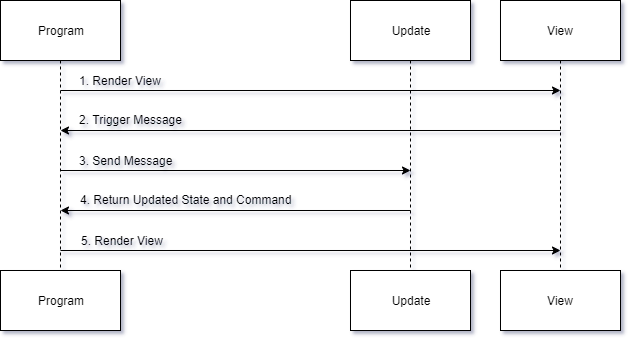
\includegraphics[height=2.5in, width=3in]{dispatchloop}
\caption{The main Elmish dispatch loop.}\label{dispatchloop}\end{figure}

Elmish is a package for Fable applications which enables the developer to utilize a ``model view update`` style of architecture. This style of application flow was popularized by the Elm Architecture for designing interactive programs. Elmish provides Fable with the core abstractions necessary to follow the Elm design style. This allows us to develop a solid core application that is largely UI-independent and easily reusable. 

Figure~\ref{dispatchloop} shows the main dispatch loop for the Elmish architecture. The page is instantiated with an initial model which is rendered by the \texttt{View} function. Once the application catches an event trigger, it sends a message through the main program to the \texttt{Update} function. This, in turn, creates a new state for the application with any additional commands and sends it back to the program for an updated render.

This structure is made possible through the Elmish abstractions of the Elm architecture. Table~\ref{tab:translate} shows how these concepts are translated into the Elmish package. The core of the application is centered around the \texttt{Model} which contains an immutable data structure representing a snapshot of the system. This model is updated whenever a new message is received in the \texttt{Update} function. The \texttt{View} method is then able to create or modify any aspects of the \textsc{UI} that have changed since the last update with the help of a renderer, like React. The \texttt{Program} then wraps this all together to produce a view from the model.

\begin{table}
  \caption{Elm concepts translated to Elmish.}
  \begin{tabular}{p{1cm}p{6cm}}
    \toprule
    \multicolumn{1}{c}{\textbf{Concept}} &
    \multicolumn{1}{c}{\textbf{Elmish Translation}} \\
    \midrule
     \verb|Model|&Immutable application state.\\
     \verb|Message|&Discriminated union representing a change of state.\\
	 \verb|Command|&Carrier of instructions.\\
     \verb|Init|&Produces initial state and commands.\\
     \verb|Update|&Produces new state given the previous state and commands.\\
     \verb|View|&Renders a declaratively built \textsc{UI}.\\
     \verb|Program|&Combines the above to produce the interface.\\
  \bottomrule
\end{tabular}
\label{tab:translate}
\end{table}

\subsection{React Components in Fable}

The \texttt{View} function depends on a renderer library to implement the actual \textsc{UI}. This makes the core program independent of any particular framework and provides large reusability to Elmish applications. The application can even run entirely without a \textsc{UI} if desired. Currently, only React and React Native have been implemented in Fable for rendering. Since our application is for the web, we used React to render our \textsc{UI} components.

Two of the most important features of React our application utilizes are function components and hooks. Function components are actual entities in the Document Object Model (DOM) of the application, meaning we can set triggers for different stages of a component's life cycle. In combination with React's hooks, we can completely manipulate components based on user initiated events and the current DOM state. 

Listing~\ref{component} shows an example of a function component. In this example, the main application component checks the internal state of the model. If the application is currently loading tournaments, then it renders a \texttt{fallback} component. Otherwise, the application will pattern match against the \textt{CurrentRoute} and load the appropriate page. This is piped into the \texttt{layout} function which defines the overall \textsc{UI} structure. The function component is utilized here to skip the rendering of a component if its props have not changed.

\begin{lstlisting}[language=F#, caption=Function component example., label=component]
let App =
    FunctionComponent.Of (fun () ->
        let model = useModel()
        if model.IsLoadingTournaments then
            fallback
        else
            match model.CurrentRoute with
            | Some(Route.Root) ->
                HomePage()
            | Some(Route.Tournaments _) ->
                TournamentsPage()
            | Some(Route.Detail _) ->
                DetailPage()
            | None ->
                h1 [] [str "404"]
        |> layout
    , "App")
\end{lstlisting}

\subsection{Python \textsc{GraphQL} Queries}

The tournament data for the web application is collected through Python \textsc{GraphQL} queries to the smash.gg \textsc{API}. Listing~\ref{query} shows a simple \textsc{GraphQL} query.

\begin{lstlisting}[language=Python, caption=Python \textsc{GraphQL} query example., label=query]
result = client.execute('''
query TournamentsByLocation() {
  tournaments(query: {
    perPage: 10
    filter: {
      location: {
        distanceFrom: "30,-81",
        distance: "50mi"
      },
      past: false,
      videogameIds: [
        1, 2, 3, 4, 5
      ]
    }
  }) {
    nodes {
      id
      }
}}}'''
\end{lstlisting}

This query retrieves the \texttt{id} of up to ten tournaments at a maximum distance of fifty miles from 20$^{\circ}$ latitude and -81$^{\circ}$ longitude. In the actual application, more properties of the \texttt{tournament} object are retrieved and the following fields are parameterized: \texttt{perPage}, \texttt{coordinates}, and \texttt{radius}. Once this query is received, the Python script converts the \textsc{GraphQL} objects to a \textsc{JSON} format and writes them to a file. This is done once during the application's startup. 

\subsection{The Smash Search Application}

The web application, dubbed Smash Search, is bundled and deployed locally using the Webpack JavaScript module bundler. A Windows command-line script is used to start the application. This script runs the Python \textsc{GraphQL} queries to load the data into a \textsc{JSON} file and boots up a local server for the web application. The user can then navigate through three different page layouts on the Smash Search application. The first is the \textit{Home} page, which only contains a button to the \textit{Tournaments} page.

The \textit{Tournaments} page reads the data from the \textsc{JSON} file, converts the objects into F$^{\sharp}$ data types, and displays the tournament information in two lists. The top-most list displays upcoming tournaments ordered from the earliest starting date to the latest starting date. The bottom-most list displays tournaments which have already completed ordered from earliest completion date to latest completion date. Each tournament entry displays the tournament's name, venue address, and starting date. Figure~\ref{smashsearch} shows an example \textit{Tournaments} page. Every tournament listing can be selected by the user to display more information.

Selecting a tournament will bring the user to the \textit{Detail} page for that specific tournament. Here, more in-depth information is displayed about the tournament. A link to the smash.gg page for the tournament is also provided.

\begin{figure}

\includegraphics[height=2.0in, width=3in]{smashsearch}
\caption{An example \textit{Tournaments} page display.}\label{smashsearch}\end{figure}

\section{Conclusion}

We presented a F$^{\sharp}$ web application which displays the Super Smash Brothers tournament information. The Fable compiler was used to convert F$^{\sharp}$ code into JavaScript and Webpack was used to bundle the required modules. The Smash Search application followed the Elm Architecture for interactive programs by utilizing the Elmish package. Python \textsc{GraphQL} queries gathered tournament data from the smash.gg \textsc{API}.

This project proved to be a good introduction into the functional paradigm for web development, but it lends itself to additional features. One such feature is the consolidation of the back-end and front-end processes. It would be beneficial to make the \textsc{GraphQL} queries from the F$^{\sharp}$ application instead of from a separate Python script. This would enable the user to input different locations during each session rather than having to recompile every time. Another feature is the option to sort tournaments by different fields. Currently, they are only sorted by date but giving the user the capability to sort by location, number of entrants, and game type would be helpful for larger data sets.

\balance

\bibliographystyle{ACM-Reference-Format}
\bibliography{berkshiret1-paper}

\end{document}
